% IEEE Cloud Computing cut of Serverless Control Plane, Container Data Plane.

\documentclass[10pt,journal]{IEEEtran}
\IEEEoverridecommandlockouts

\usepackage{microtype}
\usepackage[T1]{fontenc}
\usepackage[utf8]{inputenc}
\usepackage{url}
\usepackage{xurl}
\usepackage{xcolor}
\definecolor{causifyblue}{HTML}{0369A1}
\usepackage{tikz}
\usepackage{tabularx}
\usepackage{booktabs}
\usepackage[font=small,labelfont=bf]{caption}
\usepackage[colorlinks=true, urlcolor=causifyblue, linkcolor=black, citecolor=black]{hyperref}
\usepackage{graphicx}
\usetikzlibrary{arrows.meta, positioning, fit, calc}
\usepackage{lettrine}
\usepackage{enumitem}
\usepackage{amsmath}
\usepackage{amssymb}
\usepackage{listings}

\lstset{
  basicstyle=\fontsize{6.5}{7.8}\selectfont\ttfamily,
  backgroundcolor=\color{gray!10},
  keywordstyle=\color{causifyblue},
  morekeywords={def,return,True,False,None,import,from,class,if,else,for,in,not,and,or,lambda,with,as,raise,try,except},
  frame=none,
  xleftmargin=0pt, xrightmargin=0pt,
  breaklines=true, breakatwhitespace=false,
  keepspaces=true, columns=flexible
}

\setlength{\emergencystretch}{2em}
\AtBeginDocument{\raggedbottom}

\newenvironment{authorbio}[1]{%
  \par\vspace{4pt}%
  \noindent{\small\textbf{#1}}\ \small\ignorespaces%
}{\par\vspace{0pt}}

\newcommand{\system}{the platform}
\newcommand{\viewas}{view-as}
\newcommand{\code}[1]{{\small\texttt{\textcolor{causifyblue}{#1}}}}

\begin{document}

\title{Serverless Control Plane, Container Data Plane:\
A Governance Boundary for Multi-Tenant SaaS Platforms}

\author{Shayan Ghasemnezhad, Giacinto Paolo (GP) Saggese, Paul Smith, Heanh Sok, and Vedanshubhai Joshi}

\markboth{IEEE Cloud Computing}{Ghasemnezhad et al.: Control Plane}
\maketitle

\begin{abstract}
Multi-tenant AI platforms often spread governance through every service. One handler validates identity, another trusts a schema prefix, and a generated API spec exposes modules a tenant never licensed. We present a production pattern that moves identity materialization, tenant scope derivation, module gating, API-surface filtering, and auditable view-as support into a serverless control plane. Container workloads on Kubernetes, Lambda-backed modules, and Fargate jobs execute only inside injected scope. In eight months at Causify AI, the pattern concentrated shared governance in a 135-line Lambda middleware spine, covered 12 data-plane services, moved five of six tenant lifecycle operations out of deployments, and reduced visible API surface by 67--90\% for limited-module tenants. Full materialization was 856 ms P50; ETag revalidation handled 91\% of steady-state traffic at 68 ms P50.
\end{abstract}

\begin{IEEEkeywords}
multi-tenant SaaS, authorization, serverless architecture, control plane,
scope injection, confused deputy, API governance, AWS Lambda, Kubernetes
\end{IEEEkeywords}

\section{Introduction}

\lettrine[lines=2, lhang=0.1, loversize=0.05]{M}{}ulti-tenant platforms grow by adding tenants, modules, support workflows, and workloads. Each addition expands the governance surface: who is calling, which tenant context is effective, which modules are licensed, which routes should exist, and which database scope a job should use. The usual path is local convenience. A service validates one claim. A worker trusts one parameter. A generated API document exposes one extra module. The product keeps moving, while governance quietly spreads into every corner of the runtime.

This paper describes a production architecture built around a hard boundary.

\begin{itemize}[label=\textbullet, leftmargin=1.2em, topsep=2pt, itemsep=1pt, parsep=0pt]
  \item \textbf{Serverless control plane:} owns governance decisions.
  \item \textbf{Container data plane:} executes workloads inside injected scope.
\end{itemize}

The boundary is structural, not aspirational. The data plane does not own tenant lookup, module registry, API-surface filtering, or impersonation allow-lists. Those live in the control plane. The AWS SaaS Lens recommends control/data-plane separation for SaaS architectures~\cite{aws_saas_lens}; this paper shows one concrete way to make the separation load-bearing.

The contributions are practical:

\begin{itemize}[label=\textcolor{causifyblue}{\textbullet}, leftmargin=1.2em, topsep=2pt, itemsep=1pt, parsep=0pt]
  \item Three recurring governance failures: scope ambiguity, governance scatter, and surface drift.
  \item A control-plane design that combines OIDC-style identity materialization, ABAC-style scope derivation, module-gated routing, OpenAPI filtering, and auditable \viewas{}.
  \item Production evidence across 12 data-plane services, including latency, endpoint exposure, lifecycle-operation cost, and audit limitations.
\end{itemize}

\section{Governance Failures}

\textbf{Scope ambiguity.} Services receive tenant identifiers from callers and treat them as truth. OWASP rates broken object-level authorization as the top API security risk~\cite{owasp_top10}; NIST SP 800-162 recommends authorization decisions derived from verified attributes, not caller assertions~\cite{nist_sp800162}. The gap between those principles and ``trust the header'' implementations produces tenant-confusion incidents.

\textbf{Governance scatter.} Every new service copies some version of identity resolution, module gating, and audit logging. With 12 data-plane services, one governance rule change becomes 12 changes. That is how policy turns into folklore.

\textbf{Surface drift.} Generated API documents often expose every route the platform knows, not every route the effective tenant may use. Clients discover disabled modules, call them, and get errors. Security sees attack surface. Support sees tickets.

These failures motivate five design goals:

\begin{itemize}[label=\textcolor{causifyblue}{\textbullet}, leftmargin=1.2em, topsep=2pt, itemsep=1pt, parsep=0pt]
  \item \textbf{G1 Explicit tenancy:} actor and effective tenant are always distinct fields.
  \item \textbf{G2 Scope injection:} scope flows downstream from the control plane, never upstream from callers.
  \item \textbf{G3 Minimized surface:} tenants see only the endpoints they have licensed.
  \item \textbf{G4 Auditable impersonation:} support can view as a tenant without shared credentials.
  \item \textbf{G5 Governance as data:} routine policy changes do not require code deployments.
\end{itemize}

\section{Architecture}

Figure~\ref{fig:arch_overview} shows the boundary. The control plane is API Gateway~\cite{aws_api_gateway}, Lambda~\cite{aws_lambda_docs}, Cognito, and DynamoDB. The data plane is EKS services, module Lambdas, Fargate jobs, and tenant-scoped storage.

\begin{figure*}[!t]
  \centering
  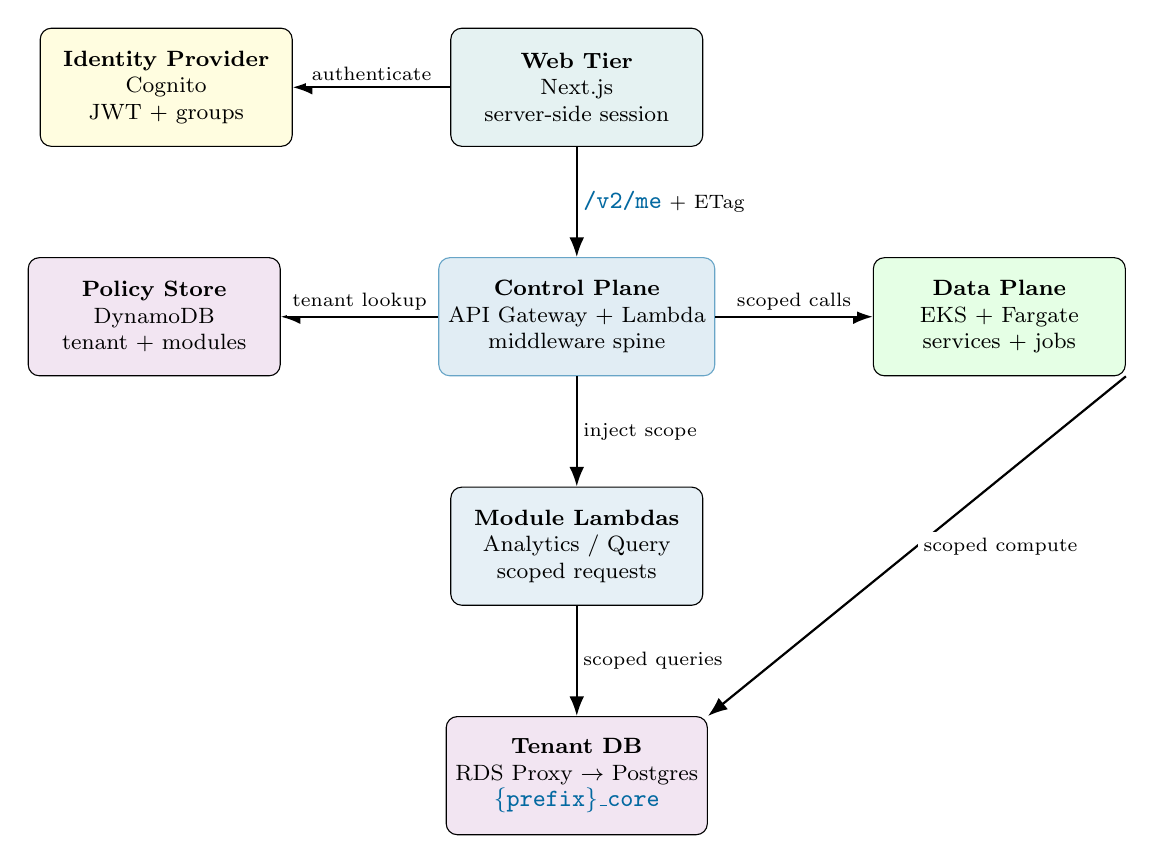
\begin{tikzpicture}[
    node distance=14mm and 20mm,
    box/.style={draw, rectangle, rounded corners, align=center,
                minimum width=32mm, minimum height=15mm,
                font=\footnotesize, fill=gray!8},
    arrow/.style={-{Latex[length=2.5mm]}, thick},
    lbl/.style={font=\scriptsize, fill=white, inner sep=2pt, align=center}
  ]
    \node[box, fill=yellow!12] (idp)
      {\textbf{Identity Provider}\\Cognito\\JWT + groups};
    \node[box, fill=teal!10, right=20mm of idp] (web)
      {\textbf{Web Tier}\\Next.js\\server-side session};
    \node[box, fill=causifyblue!12, draw=causifyblue!60, below=14mm of web] (cp)
      {\textbf{Control Plane}\\API Gateway + Lambda\\middleware spine};
    \node[box, fill=violet!10, left=20mm of cp] (ddb)
      {\textbf{Policy Store}\\DynamoDB\\tenant + modules};
    \node[box, fill=causifyblue!10, below=14mm of cp] (modlam)
      {\textbf{Module Lambdas}\\Analytics / Query\\scoped requests};
    \node[box, fill=green!10, right=20mm of cp] (dp)
      {\textbf{Data Plane}\\EKS + Fargate\\services + jobs};
    \node[box, fill=violet!10, below=14mm of modlam] (rds)
      {\textbf{Tenant DB}\\RDS Proxy $\rightarrow$ Postgres\\\code{\{prefix\}\_core}};

    \draw[arrow] (web.west) -- node[lbl,above] {authenticate} (idp.east);
    \draw[arrow] (web.south) -- node[lbl,right] {\code{/v2/me} + ETag} (cp.north);
    \draw[arrow] (cp.west) -- node[lbl,above] {tenant lookup} (ddb.east);
    \draw[arrow] (cp.south) -- node[lbl,right] {inject scope} (modlam.north);
    \draw[arrow] (cp.east) -- node[lbl,above] {scoped calls} (dp.west);
    \draw[arrow] (modlam.south) -- node[lbl,right] {scoped queries} (rds.north);
    \draw[arrow] (dp.south east) -- node[lbl,right] {scoped compute} (rds.north east);
  \end{tikzpicture}
  \caption{The control plane resolves identity, effective tenant context, module capability, API surface, and downstream scope. The data plane executes within injected scope.}
  \label{fig:arch_overview}
\end{figure*}

\textbf{The identity contract.} The control plane exposes \code{/v2/me}, a versioned contract similar to an OpenID Connect UserInfo endpoint~\cite{oidc_core}. It returns actor identity, effective context, derived signals such as \code{schema\_prefix}, and allowable impersonation targets. The schema prefix belongs to the effective context. When support uses \viewas{}, the actor remains the support engineer; the effective tenant changes.

The endpoint supports ETag and \code{If-None-Match} semantics under RFC 9110~\cite{rfc9110}. Identity is cheap to revalidate and expensive only when it changes.

\section{Control Plane Design}

The Lambda is built around four pillars.

\textbf{Middleware spine.} All handlers pass through the same authentication, response-header, and ETag middleware chain. The spine validates Cognito JWTs, resolves tenant membership from the platform table, derives role and \code{schema\_prefix}, builds impersonation allow-lists, and applies security headers.

\textbf{Scope injection.} Tenant scope is derived exclusively from the tenant record, never from headers or query parameters. The control plane injects \code{schema\_prefix} into downstream Lambda and job payloads. Downstream services reject missing or malformed scope; they do not decide which tenant a caller belongs to.

\textbf{Module gating and surface minimization.} Each route carries a module requirement such as \code{@requires\_module("grid")}. The control plane rejects missing modules before handler execution. The \code{/v1/openapi.json} endpoint filters paths by the effective tenant's enabled-module set and prunes unreferenced schemas.

\textbf{Auditable impersonation.} The \viewas{} mechanism lets operators view as a tenant without shared accounts. The \code{X-View-As} payload is allow-listed server-side, signed with HMAC-SHA256, bound to a nonce, stored in an encrypted server-side session, and revoked on logout or tenant switch. The browser never receives the signing key. If nonce registration fails, activation fails closed.

\section{Data Plane Integration}

The data plane runs Amazon EKS services, module Lambdas, Airflow-driven workflows, and ECS/Fargate jobs. Long-running workloads include Optima-style portfolio optimization, DataMap pipeline orchestration, and scheduled analytics. The control plane calls into the data plane; the data plane does not call back to resolve governance.

Database credentials are managed through AWS Secrets Manager and RDS Proxy. Per-tenant isolation uses PostgreSQL schemas. Module Lambdas set \code{search\_path = '\{prefix\}\_core'} after validating \code{schema\_prefix}. Validation protects against malformed strings. It does not replace authoritative derivation.

Fargate jobs receive tenant scope at launch through the ECS \code{RunTask} payload~\cite{ecs_runtask}. No per-job identity resolution occurs. Jobs are data-plane executions with longer time budgets, not exceptions to the governance model.

\section{Defense-in-Depth}

The threat model focuses on forged tenancy context, confused-deputy scope substitution~\cite{confused_deputy}, disabled-endpoint discovery, and operator damage during impersonation. Five controls make those failures harder.

\begin{enumerate}[leftmargin=1.2em, topsep=2pt, itemsep=2pt, parsep=0pt]
  \item JWT validation is required, but tenant scope is re-derived from membership state.
  \item \viewas{} is allow-listed, signed, nonce-bound, and attributable.
  \item Scope is injected downstream and missing scope is rejected.
  \item Unlicensed endpoints disappear from the served API spec and return \code{403} if called directly.
  \item Network and transport hardening prevent public shortcuts around compute and data stores.
\end{enumerate}

The policy store is now a critical surface. That is the trade. Moving governance from code to data makes tenant operations faster, but a bad policy write can hurt. Policy-store writes therefore need scoped IAM, review, schema validation, and audit logs.

\section{Evaluation}
\label{sec:eval}

All measurements come from one production deployment at Causify AI.

\textbf{Latency.} Table~\ref{tab:latency} reports \code{/v2/me} full-materialization latency from 1,368 production observations at 512 MB Lambda memory, collected from CloudWatch metrics during March--April 2026.

\begin{table}[h!]
  \centering
  \caption{\code{/v2/me} full-materialization latency at 512 MB.}
  \label{tab:latency}
  \small
  \begin{tabularx}{\columnwidth}{X r}
    \toprule
    \textbf{Metric} & \textbf{ms} \\
    \midrule
    P50 & 856 \\
    P75 & 938 \\
    P90 & 1,038 \\
    P95 & 1,112 \\
    P99 & 1,176 \\
    \bottomrule
  \end{tabularx}
\end{table}

ETag revalidations return \code{304 Not Modified} at 68 ms P50 and account for 91\% of steady-state requests. At that hit rate, amortized per-page cost is about 139 ms. Cold starts add 300--600 ms in observed tail cases; Provisioned Concurrency is available when needed~\cite{aws_lambda_docs}.

\textbf{Scope confusion.} CI checks that route handlers apply module requirements and that Lambdas receiving \code{schema\_prefix} reject missing values. Runtime logs emit actor tenant, effective tenant, and schema prefix. Within this detection envelope, structured-log correlation found zero actor/effective-tenant mismatches over eight months of production operation. The method cannot detect a wrong tenant derivation if the control plane derives the wrong value consistently.

\textbf{Surface reduction.} Table~\ref{tab:surface} shows endpoint exposure across synthetic module tiers from a 48-endpoint surface.

\begin{table}[h!]
  \centering
  \caption{Endpoint exposure after OpenAPI filtering.}
  \label{tab:surface}
  \small
  \begin{tabularx}{\columnwidth}{X r r}
    \toprule
    \textbf{Modules enabled} & \textbf{Visible} & \textbf{Reduction} \\
    \midrule
    0 (core only) & 5  & 90\% \\
    1             & 16 & 67\% \\
    2             & 27 & 44\% \\
    3+            & 38 & 21\% \\
    Full access   & 48 & 0\% \\
    \bottomrule
  \end{tabularx}
\end{table}

\textbf{Governance concentration.} Shared governance lives in a 135-line Lambda middleware spine. Reimplementing comparable logic across 12 services would place roughly 1,620 lines on the wrong side of the boundary. Five of six common tenant lifecycle operations are policy-store updates taking under five minutes. Adding a new module type still requires code. Migration of the 12 services took roughly 160 engineer-hours across two sprints.

\section{Related Work and Limits}

NIST ABAC~\cite{nist_sp800162}, OPA~\cite{opa_docs}, Cedar~\cite{cedar_docs}, and Zanzibar~\cite{zanzibar} provide authorization models and policy systems. Our design is narrower. It materializes tenant context once and injects scope into services that should not rediscover it.

Service meshes such as Istio and Linkerd enforce network-layer authorization~\cite{istio_authz}. They are valuable but do not replace tenant-aware OpenAPI filtering, module-gated routing, or database schema-prefix injection.

The limits are real. The implementation is AWS-specific. The decorator approach is Python-specific. Surface filtering is REST-first. The evaluation is a single-organization case study. And the control plane remains load-bearing: if it derives scope incorrectly, downstream services cannot prove the mistake.

\section{Conclusion}

The bug that hurts a multi-tenant platform is often ordinary: a missing scope field, a stale spec, an endpoint that exists when it should not, a job that runs under the wrong tenant. The platform does not collapse. It just becomes less trustworthy.

A serverless control plane paired with a container data plane gives those failures one place to be prevented, reviewed, and logged. The control plane decides and attests. The data plane executes. That boundary is not a silver bullet, but it made governance less scattered, tenant changes cheaper, API exposure smaller, and incident analysis calmer.

\noindent\textbf{Takeaways for Practitioners}
\begin{itemize}[label=\textbullet, leftmargin=1.2em, topsep=2pt, itemsep=1pt, parsep=0pt]
  \item \textbf{Materialize identity as a versioned contract.} Expose actor, effective tenant, modules, impersonation, and scope in one response. Cache with ETag/304.
  \item \textbf{Derive and inject scope.} Resolve \code{schema\_prefix} from tenant state and reject downstream calls that omit it.
  \item \textbf{Filter API surface at the boundary.} Prune OpenAPI paths by enabled modules. Keep backend authorization as the final barrier.
\end{itemize}

\bibliographystyle{IEEEtran}
\bibliography{references}

\section*{About the Authors}

\begin{authorbio}{Shayan Ghasemnezhad}
is Infrastructure and DevOps Lead at Causify AI, Turin, Italy. His research interests include platform engineering and cloud solutions architecture, production AI/ML systems, and secure, reliable infrastructure operations. Ghasemnezhad received his Bachelor's degree in Digital Management from Ca' Foscari University of Venice. Contact him at shayan@causify.ai.
\end{authorbio}

\begin{authorbio}{Giacinto Paolo (GP) Saggese}
is Co-founder and CTO at Causify AI, Potomac, Maryland, USA. His research interests include machine learning, fintech, and the commercialization of research. Saggese received his Ph.D. degree in Electrical and Computer Engineering from the University of Illinois Urbana-Champaign. He is an Adjunct Professor at the University of Maryland, College Park. Contact him at gp@causify.ai.
\end{authorbio}

\begin{authorbio}{Paul Smith}
is Co-founder and Chief Scientist at Causify AI, Cary, North Carolina, USA. His research interests include causal inference, Bayesian modeling, and time-series prediction. Smith received his Ph.D. degree in Mathematics from UCLA. Contact him at paul@causify.ai.
\end{authorbio}

\begin{authorbio}{Heanh Sok}
is Software Engineer at Causify AI, College Park, Maryland, USA. His research interests include big data systems, distributed systems, and AI/ML engineering and operations. Sok received his Master's degree in Data Science from the University of Maryland, College Park. Contact him at h.sok@causify.ai.
\end{authorbio}

\begin{authorbio}{Vedanshubhai Joshi}
is Software Engineer at Causify AI, Indiana, USA. His research interests include platform infrastructure, multi-tenant API design, and data engineering pipelines. Joshi received his Master's degree in Computer Science from Purdue University. Contact him at v.joshi@causify.ai.
\end{authorbio}
\end{document}
